Nous allons introduire le groupe fondamental, un outil de topologie algébrique, invariant par homéomorphisme. Intuitivement, nous pouvons le voir comme un outil permettant d'étudier le comportement des lacets (voir définition \ref{def:loops}) sur un espace pointé. Cet outil nous permettra de démontrer que la sphère et le tore ne sont pas homéomorphes : l'idée sous-jacente étant que les lacets de la sphère peuvent se contracter en un point (voir figure \ref{fig:lacet-sphere}), tandis que ceux du tore faisant le tour du "trou" en sont incapables (voir figure \ref{fig:lacet-tore}).

\begin{figure}[H]
\centering
\begin{subfigure}[c]{0.6\linewidth}
\centering
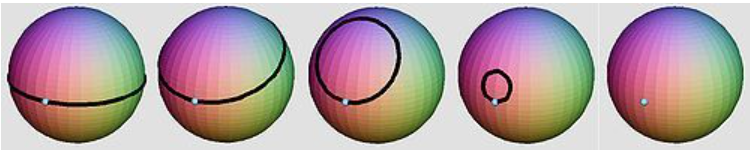
\includegraphics[width=0.7\linewidth]{pictures/sphere-intro.png}
\caption{Lacet de la sphère qui se rétracte}
\label{fig:lacet-sphere}
\end{subfigure}
\begin{subfigure}[c]{0.3\linewidth}
\centering
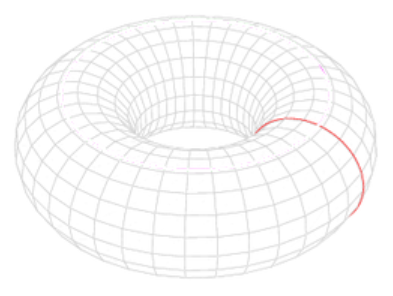
\includegraphics[width=0.7\linewidth]{pictures/tore-intro.png}
\caption{Lacet "coincé" du tore}
\label{fig:lacet-tore}
\end{subfigure}
\end{figure}

Ce chapitre est décomposé en trois grandes sections : \begin{enumerate}
    \item La construction du groupe fondamental, où nous démontrons notamment qu'il possède une structure de groupe (d'où son nom). Nous démontrons ensuite qu'il s'agit d'un invariant par homéomorphisme, et par conséquent qu'il permet de discriminer les espaces. Nous démontrons ainsi que la sphère et le tore ne peuvent être homéomorphes.
    \item Le groupe fondamental du cercle. Sa caractérisation n'est pas si trivial qu'il n'y paraît, et implique notamment l'introduction des revêtements. Suite à ce résultat, nous arrivons à caractériser plusieurs autres groupes fondamentaux.
    \item Les revêtements possèdent un lien encore plus puissant avec les groupes fondamentaux. En particulier, il existe une correspondance de Galois entre les sous-groupes du groupe fondamental et les revêtements de l'espace à isomorphisme près. La démonstration de cette correspondance n'étant pas triviale, elle est découpée en plusieurs parties. 
\end{enumerate}

Sur l'ensemble du chapitre, nous avons semé des exemples simples, apportant une illustration aux propos énoncés.

\section{Un groupe fondamental ?}

Dans cette première section, nous allons définir le groupe fondamental, et démontrer qu'il possède une structure de groupe. Pour cela, nous nous introduisons les lacets, et s'intéresser à eux selon une relation d'équivalence, nommée homotopie.

\begin{definition}\label{def:loops}
Un \emph{lacet}, ou une \emph{boucle}, est un chemin ayant le même point de départ et d'arrivée. Plus formellement, il s'agit d'une application~$\gamma:[0,1]\to X$ telle que~$\gamma(0)=\gamma(1)$. Nous appelons \emph{point de base} le point de départ et d'arrivée du lacet.
\end{definition}

Un lacet est un chemin, il possède donc également une direction, allant de $\gamma(0)$ à $\gamma(1)$.

\begin{exemple}
En considérant le cercle $\s{1}$ dans le plan complexe, le chemin défini par $t\mapsto e^{2i\pi t}$ est un lacet ayant pour point de base~$(1,0)$.
\end{exemple}

L'exemple suivant est important, car introduit le concept de \emph{polygone fondamental}, omniprésent en topologie algébrique, et par conséquent dans ce mémoire. Cette représentation est dite intrinsèque, car ne dépend d'aucun espace environnant. Celle-ci est aux antipodes de leurs plongements dans certains espaces euclidiens~$\bb{R}^n$, même s'il existe un homéomorphisme entre les deux représentations \cite{Homeo-article}.

\begin{exemple}
La figure \ref{tkz:mobius} est la représentation du polygône fondamental du ruban de Mobiüs, un carré avec une identification de deux côtés opposés via une torsion (les deux flèches vont dans deux sens différents).
\begin{figure}[H]
\centering
\begin{subfigure}[b]{0.45\linewidth}
\centering
\begin{tikzpicture}
    % Background color
    \fill[gray!30] (0,0) rectangle (4,4);

    % Top arrow with label A
    \draw[thick, red, ->, >=stealth'] (0,4) -- (4,4) node[midway, below] {\textbf{A}};

    % Bottom arrow with label A
    \draw[thick, red, ->, >=stealth'] (4,0) -- (0,0) node[midway, above] {\textbf{A}};

    % Outer rectangle
    \draw[black, line width=.0mm] (0,0) rectangle (4,4);
\end{tikzpicture}
\caption{Ruban de Mobius}
\label{tkz:mobius}
\end{subfigure}
\begin{subfigure}[b]{0.45\linewidth}
\centering
\begin{tikzpicture}
    % fond gris
    \fill[gray!30] (0,0) rectangle (4,4);
    %flèche du haut
    \draw[thick, red, ->, >=stealth'] (0,4) -- (4,4) node[midway, below] {\textbf{A}};
    %flèche du bas
    \draw[thick, red, ->, >=stealth'] (4,0) -- (0,0) node[midway, above] {\textbf{A}};
    %carré
    \draw[black, line width=.0mm] (0,0) rectangle (4,4);
    
    %gamma'
    \draw[thick, black, ->] (3,0) -- (2.5,1);
    \draw[thick, black] (2.5,1) -- (2,2) node[near start, left] {$\gamma'$};
    \draw[thick, black, ->] (2,2) -- (1.5,3);
    \draw[thick, black] (1.5,3) -- (1,4);

    %gamma
    \draw[thick, ->] (3.4, 2) arc[start angle=0, end angle=360, radius=0.7] node[right] {$\gamma$};
    % Point at (2,2)
    \filldraw[black] (2,2) circle (2pt) node[right] {$x_0$};
\end{tikzpicture}
\caption{Ruban de Mobius et deux lacets}
\label{tkz:mobius-loops}
\end{subfigure}
\end{figure}

Nous pouvons tracer une infinité de lacet sur le ruban, mais deux grandes "familles" en ressortent, illustrés dans la figure \ref{tkz:mobius-loops} : les lacets qui restent dans l'intérieur du carré (comme le lacet $\gamma$), et les lacets qui utilisent l'identification $A$ des côtés (comme le lacet $\gamma'$).
\end{exemple}

\subsection{Homotopie}\label{sec:homotopy}

L'homotopie est la formalisation de l'idée de la déformation d'objets, en particuliers des chemins et lacets sur un espace. L'idée du raccoursissement de lacet devient ainsi représentable topologiquement parlant.

\begin{definition}\label{def:homotopy-paths}
Soient $x_0, x_1$ deux points de l'espace $X$, et soient $\gamma_0$ et $\gamma_1$ deux chemins partageant les mêmes extrémités $x_0$ et $x_1$. Une \emph{homotopie} entre $\gamma_0$ et $\gamma_1$ est une application $\Gamma:[0,1]^2\to X$, définie par $\Gamma(t,s)=\gamma_t(s)$, continue en $t$ et telle que, pour tout $t\in[0,1]$, $\gamma_t(0)=x_0$ et $\gamma_t(1)=x_1$.

Intuitivement, cela revient à dire qu'il existe une famille $\gamma_t$ de chemin fixant les extrémités, et continue en $t$. Nous disons alors que $\gamma_0$ est homotope à $\gamma_1$, ou bien que $\gamma_0$ et $\gamma_1$ sont homotopes, et l'on note $\gamma_0\simeq\gamma_1$.
\end{definition}

\begin{figure}[H]
    \centering
    \begin{tikzpicture}
    % Points A et B
    \filldraw[black] (0,0) circle (2pt) node[above left] {$x_0$};
    \filldraw[black] (6,0) circle (2pt) node[above right] {$x_1$};
    % t=0
    \draw[thick, ->, >=stealth] (0,0) .. controls (1.5,0.8) .. (3,1) node[near end, above] {$\gamma_0$}; 
    \draw[thick] (3,1) .. controls (4.5,0.8) .. (6,0);
    %t=.25
    \draw[dashed, ->, >=stealth'] (0,0) .. controls (1.5,0.4) .. (3,0.5); 
    \draw[dashed] (3,0.5) .. controls (4.5,0.4) .. (6,0);
    %t=0.5
    \draw[thick, dashed, ->, >=stealth'] (0,0) -- (3,0)  node[near end, above] {$\gamma_{\frac{1}{2}}$}; 
    \draw[thick, dashed] (3,0) -- (6,0);
    %t=.75
    \draw[dashed, ->, >=stealth'] (0,0) .. controls (1.5,-0.4) .. (3,-0.5); 
    \draw[dashed] (3,-0.5) .. controls (4.5,-0.4) .. (6,0);
    % t=1
    \draw[thick, ->, >=stealth'] (0,0) .. controls (1.5,-0.8) .. (3,-1) node[near end, below] {$\gamma_1$}; 
    \draw[thick] (3,-1) .. controls (4.5,-0.8) .. (6,0);
\end{tikzpicture}
    \caption{Homotopie entre les chemins $\gamma_0$ et $\gamma_1$}
    \label{tkz:path-homotopy}
\end{figure}

\begin{exemple}
Dans l'espace euclidien $\bb{R}^n$, il existe toujours une homotopie linéaire entre deux chemins avec les mêmes extrémités. En effet, en notant $\gamma_0$ et $\gamma_1$ deux chemins d'extrémités communes $x_0$ et $x_1$, nous avons l'homotopie suivante, pour~$t\in[0,1]$ :  $\gamma_t(s)=(1-t)\gamma_0(s)+t\gamma_1(s)$. Il est facile de vérifier que $\gamma_t(0)=x_0$ et~$\gamma_t(1)=x_1$, pour tout $t\in[0,1]$.
\end{exemple}

Plutôt que de s'intéresser à l'ensemble des lacets, nous allons préférer les étudier à homotopie près. D'une part, il est possible dans certains cas de passer d'une infinité de lacets à un nombre fini de classes d'équivalences. Et d'autre part, les classes d'homotopie de lacets possèdent une structure naturelle de groupe. C'est ce que nous allons montrer par la suite.

\begin{proposition}
La relation d'homotopie entre chemins est une relation d'équivalence. Nous noterons $[\gamma]$ la classe d'équivalence de $\gamma$ sous la relation d'homotopie, et nous appellée \emph{classe d'homotopie} de $\gamma$.
\end{proposition}

En rappellant qu'une relation d'équivalence est définie comme étant réflexive, symétrique et associative, la démonstration consiste simplement à montrer successivement que les trois propriétés sont vérifiées par la relation d'homotopie.
\begin{proof}
\textit{(Réfléxivité)} Pour tout chemin $\gamma$ sur $X$, il existe l'homotopie constante $\gamma_t(s)=\gamma(s)$. Nous en conluons que $\gamma\simeq\gamma$.

\textit{(Symétrie)} Pour toute homotopie $\gamma_t(s)$ entre $\gamma$ et$\gamma'$, il est clair que l'homotopie $\gamma_{1-t}$ permet d'aller de $\gamma'$ vers $\gamma$. Nous en concluons que $\gamma'\simeq\gamma$.

\textit{(Associativité)} Soient $\gamma\simeq\gamma'$ et $\gamma'\simeq\gamma''$. En notant $\gamma_t$ l'homotopie entre $\gamma$ et $\gamma'$ et $\gamma_t'$ l'homotopie entre $\gamma'$ et~$\gamma''$, nous pouvons intuitivement construire l'homotopie entre $\gamma$ et $\gamma''$ en concaténant les deux homotopies précédentes. Plus formellement, nous obtenons l'homotopie suivante : \[\gamma''_t(s)= \left\{\begin{matrix}
\gamma_{2t}(s),&\text{si }t\in[0,\frac{1}{2}], \\
\gamma'_{2t-1}(s),&\text{si }t\in[\frac{1}{2},1].
\end{matrix}\right.\]Celle=ci est continue sur $[0,\frac{1}{2}]$ et $[\frac{1}{2},1]$ par définition des homotopies $\gamma_t$ et $\gamma'_t$, et en $\frac{1}{2}$ du fait que $\gamma_1=\gamma'=\gamma'_0$. L'homotopie $\gamma_t''$ va donc de $\gamma_0=\gamma$ vers~$\gamma'_1=\gamma''$. Nous en concluons ainsi que $\gamma\simeq\gamma''$.
\end{proof}

Les lacets étant des chemins, nous pouvons considérer les classes d'homotopie de ceux-ci.

\subsection{Loi de composition}

Désormais, pour pouvoir parler de groupe, nous avons besoin d'un opérateur entre les classes d'homotopie. Nous allons alors partir d'une loi de composition interne (LCI) sur les chemins qui soit compatible avec la relation d'équivalence d'homotopie.

\begin{wrapfigure}{r}{0.3\textwidth}
    \centering
    \begin{tikzpicture}
    \filldraw[black] (0,0) circle (2pt) node[above left] {$x_0$};
    \filldraw[black] (2,0.5) circle (2pt) node[above] {$x_1$};
    \filldraw[black] (3,1.7) circle (2pt) node[above left] {$x_2$};
    \draw[thick, ->, >=stealth, red] (0,0) .. controls (0.5,0) .. (1,0.05) node[near start, above] {$\gamma$}; 
    \draw[thick, red] (1,0.05) .. controls (1.5,0.2) .. (2,0.5) ; 
    \draw[thick, blue, ->, >=stealth'] (2,0.5) .. controls (2.5,0.6) .. (3,1) ; 
    \draw[thick, blue] (3,1) .. controls (3.1,1.2) .. (3,1.7) node[near end, right] {$\gamma'$};
    \node[violet] at (2,0.2) {$\gamma\cdot\gamma'$};
    \end{tikzpicture}
\end{wrapfigure}

\phantom{}
\begin{definition}
Pour $\gamma,\gamma'$ deux chemins sur un espace $X$ tels que~$\gamma(1)=\gamma'(0)$, nous pouvons définir le lacet $\gamma\cdot\gamma'$ comme étant le chemin résultat de la \emph{concaténation} de $\gamma$ et $\gamma'$. Formellement, nous le définissons comme suit : \[\gamma\cdot \gamma'(s)=\left\{\begin{matrix}
\gamma(2s)&\text{si }0\leq s\leq \frac{1}{2}\\ 
\gamma'(2s-1)&\text{si }\frac{1}{2}\leq s\leq 1.
\end{matrix}\right.\]

En particulier pour les lacets avec le même point de base, la concaténation est une loi de composition interne.
\end{definition}

%En effet, la concaténation de deux lacets donne un lacet qui passera sur le point de base à mi-parcours. Nous pouvons visualler cela avec le chiffre 8, qui est concaténation d'un lacet supérieur et un lacet inférieur, où le point de base est le point d'intersection des deux lacets.

\begin{proposition}
La LCI de la concaténation de lacets est compatible avec la relation d'homotopie. Nous définissons ainsi une LCI sur les classes d'homotopie de lacets, tel que pour $\gamma$ et $\gamma'$ deux lacets ayant le même point de base, on ait $[\gamma][\gamma']=[\gamma\cdot\gamma']$
\end{proposition}

La démonstration consiste à vérifier si, pour deux paires de lacets homotopes, la concaténation d'éléments de chaque pair est homotope à la concaténation des deux autres. Pour cela, nous allons construire l'homotopie entre les deux concaténations, à partir des homotopies de base.

\begin{proof}
Soient $\gamma\simeq\gamma'$ et $\zeta\sim\zeta'$ quatres lacets ayant un même point de base $x_0\in X$. Nous allons montrer que $\gamma\cdot\zeta\simeq\gamma'\cdot\zeta'$, ce qui suffit pour démontrer la proposition.

Notons respectivement $\gamma_t$ et $\zeta_t$ les homotopies allant de $\gamma$ vers $\gamma'$ et de $\zeta$ vers~$\zeta'$. Nous considérons l'application obtenue par concaténation de ces homotopies :$\tau_t=\gamma_t\cdot \zeta_t$. \begin{equation}\label{eq:homotopy-concatenate}
\tau_t(s)=\gamma_t\cdot\zeta_t(s)=\left\{\begin{matrix}
\gamma_t(2s)&\text{si }0\leq s\leq \frac{1}{2}\\ 
\zeta_t(2s-1)&\text{si }\frac{1}{2}\leq s\leq 1.
\end{matrix}\right.
\end{equation}Montrons que cela définit une homotopie entre $\gamma\cdot\zeta$ et $\gamma'\cdot\zeta'$. Pour $t=0$, on a $\gamma_0\cdot\zeta_0=\gamma\cdot\zeta$, et pour~$t=1$, on a $\gamma_1\cdot\zeta_1=\gamma'\cdot\zeta'$. De plus, nous avons $\gamma_t\cdot\zeta_t(0)=\gamma_t(0)=x_0$ et $\gamma_t\cdot\zeta_t(1)=\zeta_t(1)=x_0$ par définition des homotopies $\gamma_t$ et $\zeta_t$. Finalement, la continuité de l'homotopie $\gamma_t\cdot\zeta_t$ est évidente : pour $s\in[0,\frac{1}{2}]$, elle est due à celle de $\gamma_t$, et pour $s\in[\frac{1}{2},1]$, elle est due à celle de $\zeta_t$.

Nous pouvons désormais conclure que $\gamma\cdot\zeta\simeq\gamma'\cdot\zeta'$, ce qui fait que la relation d'homotopie de lacets est compatible avec la LCI de concaténation.
\end{proof}

Nous pouvons passer à la définition de cet ensemble.

\begin{definition}
L'ensemble des classes d'homotopie de lacets de $X$ basés en $x_0\in X$ est appelé le \emph{groupe fondamental} de $X$ en $x_0$, ou sur l'espace pointé $(X,x_0)$, et on note $\pi_1(X,x_0)$.
\end{definition}

Montrons que la terminologie donnée à cet ensemble est justifiée, c'est à dire de montrer qu'il s'agisse bien d'un groupe. 

\begin{theorem}
L'ensemble $\pi_1(X,x_0)$ possède une structure de groupe, avec le produit définie précédemment sur les classes de lacets.
\end{theorem}

\begin{proof}
Soit $X$ un espace et soit $x_0\in X$. Il suffit de montrer que~$\pi_1(X,x_0)$ vérifie les propriétés d'un groupe.\begin{enumerate}
    \item Soit $c$ le lacet constant en $x_0$, dont nous notons $[c]$ sa classe d'homotopie. Soit~${\alpha\in\pi_1(X,x_0)}$ une classe d'homotopie, avec $\gamma$ un représentant. Montrons que $\alpha[c]=\alpha$ et~${[c]\alpha=\alpha}$. Pour cela, il suffit de montrer que $\gamma\cdot c\simeq\gamma$ et $c\cdot\gamma\simeq\gamma$.

    Dans un premier temps, on considère l'application suivante, définie pour $t\in[0,1]$ : \[\gamma_t(s)=\left\{\begin{matrix}
    \gamma\big(2s-t\big)&\text{si }0\leq s\leq \frac{1}{2}(1+t)\\ 
    c(0)=x_0&\text{sinon},
    \end{matrix}\right.\]dont nous voulons montrer qu'il s'agit d'une homotopie entre $\gamma_0=\gamma\cdot c$ et $\gamma_1=\gamma$. Vérifions que cette application est bien définie, en montrant qu'elle est continue en $s$. Il suffit pour cela de voir que pour $s=\frac{1}{2}(1+t)$, nous avons $2s-t=1$, d'où $\gamma(2s-t)=x_0$. L'application est continue en~$t$ (ce paramètre nous sert à raccourcir l'intervalle sur lequel nous sommes sur $c$), et les extrémités sont conservées. Alors, nous pouvons en déduire que cette application est bien une homotopie entre les lacets $\gamma\cdot c$ et $\gamma$.

    Dans un second temps, on considère l'application suivante, définie pour $t\in[0,1]$ : \[\gamma'_t(s)=\left\{\begin{matrix}
    c\left(0\right)=x_0&\text{si }0\leq s\leq \frac{1}{2}(1-t)\\ 
    \gamma\left(\frac{2s+t-1}{t+1}\right)&\text{si }\frac{1}{2}(1-t)\leq s\leq 1.
    \end{matrix}\right.\] Pour $s=\frac{1}{2}(1-t)$, on a ${2s+t-1=(1-t)+t-1=0}$, d'où $\gamma\big(\frac{2s+t-1}{t+1}\big)=x_0$. Cela montre que notre application est continue. De même que précédemment, il est facile de vérifier que cela constitue une homotopie entre les lacets~$c\cdot\gamma$ et $\gamma$.

    Nous pouvons alors en conclure que la classe d'homotopie $[c]$ est l'élément neutre pour le produit de classes.
    \item Soit $\alpha\in\pi_1(X,x_0)$. Trouvons une classe d'homotopie $\beta$ telle que $\alpha\beta=[c]$. Soit $\gamma$ un lacet de point de base $x_0$ un représentant de la classe $\alpha$. En notant $\overline{\gamma}$ le lacet inverse de $\gamma$ (ie.~${\overline{\gamma}(s)=\gamma(1-s)}$), montrons que $\gamma\cdot\overline{\gamma}\simeq c$ et $\overline{\gamma}\cdot\gamma\simeq c$.

    \bigskip Dans un premier temps, on considère l'application suivante, définie pour $t\in[0,1]$ : \[\gamma_t(s)=\left\{\begin{matrix}
    \gamma\big(2s(1-t)\big)&\text{si }0\leq s\leq \frac{1}{2}\\ 
    \overline{\gamma}\big((2s-1)(1-t)+t\big)&\text{si }\frac{1}{2}\leq s\leq 1.
    \end{matrix}\right.\]Nous allons montrer que l'application est continue en $s$ et qu'elle fixe les extrémités. Pour cela, il faut vérifier les points suivants : \begin{enumerate}
        \item Pour $s=0$, on a $\gamma\big(2s(1-t)\big)=\gamma(0)$ ;
        \item Pour $s=1$, on a $\overline{\gamma}\big((2s-1)(1-t)+t\big)\overline{\gamma}(1-t+t)=\overline{\gamma}(1)$ ; 
        \item Pour $s=\frac{1}{2}$, nous avons d'un côté $\gamma\big(2s(1-t)\big)=\gamma(1-t)$ pour le terme du haut, et de l'autre~${\overline{\gamma}\big((2s-1)(1-t)+t\big)=\overline{\gamma}(t)=\gamma(1-t)}$ pour celui du bas.
    \end{enumerate} Ensuite, il est facile de vérifier la continuité en $t$, et que l'on a $\gamma_0=\gamma\cdot\overline{\gamma}$ et $\gamma_1=c$. Nous pouvons alors en déduire que cette application est une homotopie entre les lacets $\gamma\cdot\overline{\gamma}$ et $c$.

    \bigskip De manière similaire, nous pouvons démontrer qu'il existe une homotopie entre $\overline{\gamma}\cdot\gamma$ et~$c$. Nous pouvons alors conclure que $\gamma\cdot\overline{\gamma}\simeq c$ et $\overline{\gamma}\cdot\gamma\simeq c$, donc que $[\gamma][\overline{\gamma}]=[c]$, ainsi que $[\overline{\gamma}][\gamma]=c$.
    \item Il nous reste à démontrer l'associativité. Soient $\alpha,\beta,\delta\in\pi_1(X,x_0)$, avec comme représentants respectifs~$\gamma,\zeta,\theta$ des classes d'homotopie. Montrons que l'on a~$\gamma\cdot(\zeta\cdot\theta)\simeq(\gamma\cdot\zeta)\cdot\theta$.

    Tout d'abord, exprimons ces lacets de manière explicite : \[\begin{split}
    \gamma\cdot(\zeta\cdot\theta)(s)&=\left\{\begin{matrix}
        \gamma(2s)&\text{si }0\leq s\leq\frac{1}{2}\\
        \zeta\cdot\theta(2s-1)&\text{si }\frac{1}{2}\leq s\leq 1
    \end{matrix}\right.\\
    &=\left\{\begin{matrix}
        \gamma(2s)&\text{si }0\leq s\leq\frac{1}{2}\\
        \zeta(4s-2)&\text{si }\frac{1}{2}\leq s\leq\frac{3}{4}\\
        \theta(4s-3)&\text{si }\frac{3}{4}\leq s\leq1,
    \end{matrix}\right.
    \end{split}\]et\[\begin{split}
    (\gamma\cdot\zeta)\cdot\theta(s)&=\left\{\begin{matrix}
        \gamma\cdot\zeta(2s)&\text{si }0\leq s\leq\frac{1}{2}\\
        \theta(2s-1)&\text{si }\frac{1}{2}\leq s\leq 1
    \end{matrix}\right.\\
    &=\left\{\begin{matrix}
        \gamma(4s)&\text{si }0\leq s\leq\frac{1}{4}\\
        \zeta(4s-1)&\text{si }\frac{1}{4}\leq s\leq\frac{1}{2}\\
        \theta(2s-1)&\text{si }\frac{1}{2}\leq s\leq1.
    \end{matrix}\right.
    \end{split}\]On considère dès lors l'application suivante, définie pour $t\in[0,1]$ : \[h_t(s)=\left\{\begin{matrix}
    \gamma\left(\frac{4s}{2-t}\right)&\text{si }0\leq s\leq \frac{1}{4}(2-t)\\
    \zeta\left(4s-2+t\right)&\text{si }\frac{1}{4}(2-t)\leq s\leq \frac{1}{4}(3-t)\\
    \theta\left(\frac{4s-4}{1+t}+1\right)&\text{si }\frac{1}{4}(3-t)\leq s\leq1.
    \end{matrix}\right.\]Nous avons plusieurs choses à vérifier : \begin{itemize}
        \item Pour $s=0$, nous avons bien $h_t(0)=\gamma(0)$ et pour $s=1$, nous avons bien $h_t(1)=\theta(1)$ ;
        \item Pour $s=\frac{1}{4}(2-t)$, nous avons $\frac{4s}{2-t}=1$, ainsi que $4s-2+t=0$. On en déduit que $h_t$ est continue en ce point.
        \item Pour $s=\frac{1}{4}(3-t)$, nous avons l'égalité $4s=3-t$. Nous en déduisons d'une part que $4s-2+t=1$ et d'autre part que~${\frac{4s-4}{1+t}+1=\frac{3-t-4}{1+t}+1=-1+1=0}$, ce qui nous permet de conclure que $h_t$ est continue en ce point $s$.
        \item Nous avons $h_0=\gamma\cdot(\zeta\cdot\theta)$ et $h_1=(\gamma\cdot\zeta)\cdot\theta$, et $h_t$ est continue en $t$.
    \end{itemize}Nous pouvons alors en conclure que $h_t$ est une homotopie entre les lacets~$\gamma\cdot(\zeta\cdot\theta)$ et $(\gamma\cdot\zeta)\cdot\theta$, ce qui nous permet de conclure que le produit sur les classes d'homotopie est associatif.
\end{enumerate}Nous pouvons ainsi conclure que le groupe fondamental $\pi_1(X,x_0)$ est bien un groupe.
\end{proof}

Intuitivement, nous venons de démontrer que les classes d'homotopie ne se préoccupe pas du "temps de parcours" du lacet, seulement du trajet. Si l'on parcourt un lacet dans un sens puis dans l'autre sens, nous considérons en terme d'homotopie que cela revient à ne pas bouger.

\begin{definition}
Un espace est dit \emph{simplement connexe} si son groupe fondamental est trivial.
\end{definition}
Ce terme vient du fait que sur un espace simplement connexe, il existe une unique classe d'homotopie entre deux points de cet espace.

\subsection{Propriétés élémentaires}

Désormais que nous savons qu'il existe une structure de groupe sur un espace, il serait bien de l'utiliser. Avant de voir un exemple concret de calcul de groupe, nous allons voir quelques propriétés de base.

\begin{proposition}
Tout sous-espace convexe $X\subset\bb{R}^n$ est simplement connexe.
\end{proposition}
\begin{proof}
Comme expliqué dans l'exemple qui suit la définition \ref{def:homotopy-paths}, pour tout couple de lacet $\gamma,\gamma'$ de $(X,x_0)$, il existe toujours une homotopie linéaire~$\gamma_t=(1-t)\gamma+t\gamma'$ allant de l'un vers l'autre. Autrement dit, tout les lacets sont homotopes entre eux, il n'existe qu'une seule classe d'homotopie, celle du chemin constant.
\end{proof}

Un autre résultat important est celui du changement du point de base.

\begin{proposition}
Soit $X$ un espace, et soient $x_0,x_1\in X$ deux points reliés par un chemin. Les groupes fondamentaux $\pi_1(X,x_0)$ et $\pi_1(X,x_1)$ sont isomorphes.
\end{proposition}
\begin{proof}
Soit $\zeta$ le chemin entre $x_0=\zeta(0)$ et $x_1=\zeta(1)$. Pour un lacet~$\gamma$ de $X$ ayant pour point de base $x_0$, nous avons $\zeta\cdot\gamma\cdot\overline{\zeta}$ qui est un lacet basé en~$x_1$. Nous pouvons alors définir l'application~$\Phi:\pi_1(X,x_0)\to\pi_1(X,x_1)$, qui envoie~$[\gamma]$ sur $[\zeta\cdot\gamma\cdot\overline{\zeta}]$. Montrons que cette application est un morphisme de groupes, puis qu'elle admet un morphisme réciproque, de telle sorte que ce soit un isomorphisme.

Nous devons tout d'abord montrer que l'application est bien définie, c'est à dire pour $\gamma\simeq\gamma'$ deux lacets de $(X,x_0)$, nous avons $\zeta\cdot\gamma\cdot\overline{\zeta}\simeq\zeta\cdot\gamma'\cdot\overline{\zeta}$. En notant~$\gamma_t$ l'homotopie entre $\gamma$ et $\gamma'$, nous avons $\zeta\cdot\gamma_t\cdot\overline{\zeta}$ qui forme une homotopie entre $\zeta\cdot\gamma\cdot\overline{\zeta}$ et $\zeta\cdot\gamma'\cdot\overline{\zeta}$.

\bigskip Soient $\alpha,\alpha'\in\pi_1(X,x_0)$, montrons que $\Phi(\alpha\alpha')=\Phi(\alpha)\Phi(\alpha')$. Soient $\gamma,\gamma'$ deux lacets de $(X,x_0)$, représentants respectifs de $\alpha$ et $\alpha'$. Nous avons : \[\begin{split}
\Phi([\gamma][\gamma'])&=\Phi([\gamma\cdot\gamma'])\\
&=[\zeta\cdot\gamma\cdot\gamma'\cdot\overline{\zeta}]\\
&=[\zeta\cdot\gamma\cdot\overline{\zeta}\cdot\zeta\cdot\gamma'\cdot\overline{\zeta}]\\
&=[\zeta\cdot\gamma\cdot\overline{\zeta}][\zeta\cdot\gamma'\cdot\overline{\zeta}]\\
&=\Phi([\gamma])\Phi([\gamma']).
\end{split}\] Nous pouvons alors en déduire qu'il s'agit d'un morphisme. Désormais, on considère l'application allant de $\pi_1(X,x_1)$ vers $\pi_1(X,x_0)$ par~$\Psi:[\gamma]\mapsto[\overline{\zeta}\cdot\gamma\cdot\zeta]$. Pour la même raison que pour $\Phi$, il s'agit d'un morphisme bien définit. Il est évident que $\Phi$ et $\Psi$ sont des morphismes réciproques l'un par rapport à l'autre, puisque~$[\zeta\cdot\overline{\zeta}]=[c]$ et~$[\overline{\zeta}\cdot\zeta]=[c]$. Nous pouvons en conclure que les deux groupes sont isomorphes.
\end{proof}
\begin{remark}
Autrement dit, le groupe fondamental d'un espace connexe par arc ne dépend pas du point choisi. Nous pouvons alors négliger la notation du point de base pour de tel espace.
\end{remark}

\subsubsection{Morphisme induit}

Le premier résultat qui nous intéresse est celui de l'invariance du groupe fondamental par homéomorphisme. Cela vient du fait de la bonne propriété que possède le groupe fondamental sur les inductions de morphismes :

\begin{definition}
Soit $f:(X,x_0)\to(Y,y_0)$ une application entre deux espaces (le point $x_0$ est envoyé sur $y_0$ via $f$). Le \emph{morphisme de groupes induit} par $f$ se défini par $f_\ast:\pi_1(X,x_0)\to\pi_1(Y,y_0)$, qui à un élément $[\gamma]\in\pi_1(X,x_0)$ renvoie~$[f\gamma]\in\pi_1(Y,y_0)$. 
\end{definition}

En théorie des catégories \ref{chap:categories}, on dit que le groupe fondamental est un \emph{foncteur} entre la catégorie des espaces pointés et la catégorie des groupes. Cela signifie qu'il vérifie le théorème suivant.

\begin{theorem}
Nous avons $id_\ast=id$, et pour $f:Y\to Z, g:X\to Y$,  l'égalité $(fg)_\ast=f_\ast g_\ast$. En théorie des catégories, nous disons que le groupe fondamental est un foncteur \emph{covariant}.
\end{theorem}
\begin{proof}
Le morphisme induit par l'identité $id:X\to X$, est défini par $[\gamma]\mapsto[id(\gamma)]=[\gamma]$, ce n'est rien d'autre que l'identité.

En reprenant les notations de l'énoncé, nous avons l'égalité suivante : \[f_\ast(g_\ast([\gamma]))=f_\ast([g\gamma])=[fg\gamma]=(fg)_\ast([\gamma]).\]
\end{proof}



\begin{theorem}
Soit $X$ et $Y$ deux espaces homéomorphes, et soit $x_0\in X$. L'homéomorphisme~$f:X\to Y$ induit un isomorphisme entre les groupes fondamentaux $f_\ast:\pi_1(X,x_0)\to\pi_1(Y,f(x_0))$.
\end{theorem}
\begin{proof}
Du fait que $f$ soit une bijection, elle admet une inverse. Cette inverse induit une inverse pour $f_\ast$, d'où le fait que les groupes fondamentaux soient isomorphes.
\end{proof}

La contraposée est plus intéressante, puisqu'elle permet d'affirmer grâce au groupe fondamental si deux groupes sont non homéomorphes.

\begin{corollary}
Si deux espaces $X$ et $Y$ ne possèdent pas le même groupe fondamental, alors ils ne sont pas homéomorphes.
\end{corollary}
\begin{remark}
Attention toutefois, la réciproque n'est pas vraie, comme nous pouvons le voir juste après.
\end{remark}

\begin{proposition}\label{prop:eq-homo-same-gr-fund}
Une équivalence d'homotopie $\phi:X\to Y$ induit un isomorphisme  entre$\pi_1(X,x_0)$ et~$\pi_1(Y,\phi(x_0))$, pour tout $x_0\in X$.
\end{proposition}
\begin{proof}

\end{proof}

\begin{proposition}
Si un espace $X$ se rétracte en $A$, alors l'inclusion induit un morphisme injectif~$i_\ast:\pi_1(A,x_0)\to\pi_1(X,x_0)$. Si c'est une déformation par rétraction, alors le morphisme induit est un isomorphisme.
\end{proposition}
\begin{proof}
Soient $r:X\to A$ et $i:A\hookrightarrow X$, tels que nous avons $ri=id_A$, ce qui induit~$r_\ast i_\ast=id$. Du fait qu'avoir un inverse à gauche implique être injectif, on en déduit que $i_\ast$ est un morphisme injectif.

Une déformation par rétraction est un cas particulier d'équivalence d'homotopie, nous pouvons alors utiliser la proposition précédente.
\end{proof}

\begin{comment}
\begin{remark}
Le fait que l'on obtiennent des isomorphismes de groupes fondamentaux sur des espaces non homéomorphes posent problème sur l'efficacité de discrimination du groupe fondamental. Ce n'est pas une méthode efficace pour savoir si deux espaces sont homéomorphes, ou simplement homotopiquement équivalent, ou encore obtenu par déformation par rétraction. Un exemple facile serait le disque qui se rétracte par déformation en un point : les deux espace sont simplement connexes, mais ne sont pas homéomorphes.
\end{remark}
\end{comment}